\chapter{Fraunhoferbuiging en ruimtelijke filtering}\label{ch:b2:diffraction}

Knijp de ogen toe naar een straatlantaarn door de spleet tussen twee
vingers en de lantaarn rekt zich uit tot een band van strepen; kijk
door de fijnste telescoop naar een ster en u ziet geen punt maar een
schijfje omringd door flauwe cirkels. Licht dat door een opening gaat,
spreidt zich uit --- hoe smaller de opening, hoe wijder de spreiding
--- en geen lens kan het strakker bundelen dan die spreiding toelaat.
Dit is \emph{\omterm{def:b2:diffraction:huygens}{buiging}}, de reden waarom een microscoop geen virus kan
zien, waarom het oplossend vermogen van een telescoop met zijn
diameter groeit, en waarom een laserbundel niet evenwijdig kan
blijven. Dit hoofdstuk berekent het buigingspatroon van een opening in
het verre veld, de grens die het aan elk optisch instrument stelt, de
manier waarop het met interferentie samengaat, en het denkbeeld ---
van Abbe --- dat het brandvlak van een lens tot een plaats maakt waar
een beeld kan worden gefilterd.

\section{Het beginsel van Huygens--Fresnel en het fraunhoferregime}

\begin{definition}[Beginsel van Huygens--Fresnel]\label{def:b2:diffraction:huygens}
\index{beginsel van Huygens--Fresnel}\index{buiging}\index{fraunhoferbuiging}
Elk punt van een \omterm{def:b2:scalar-light-model:path}{golffront} (of van een opening die door een golf wordt
belicht) werkt als een tweede bron die een bolvormig golfje uitzendt, in
fase met de golf daar; de golf daarachter is de coherente som van de
golfjes. Voor een opening $\Sigma$ belicht door een vlakke golf met amplitude $a$
is de amplitude die een ver punt bereikt
$\underline s(M) = K\iint_\Sigma\eu^{-\iu\varphi(P, M)}\dd S$, met
$\varphi(P, M)$ de fase van de weg van het openingspunt $P$ naar $M$
($K$ een constante). \emph{Fraunhoferbuiging} (in het verre veld) is het geval
waarin $M$ op oneindig ligt --- of in het brandvlak van een lens --- zodat
de stralen van alle punten van de opening naar $M$ evenwijdig zijn, in
de richting $\vect u$, en
\[
\varphi(P, M) = \varphi_0 - \frac{2\pi}\lambda\,\vect{OP}\cdot\vect u , \qquad
\underline s(\vect u) \propto \iint_\Sigma\eu^{\iu(2\pi/\lambda)\vect{OP}\cdot\vect u}\dd S .
\]
Het patroon wordt op oneindig waargenomen, of in het brandpunt $F'$ van een lens,
waar de richting $\vect u$ met kleine hoeken $(\alpha, \beta)$ op het
punt $(f\alpha, f\beta)$ wordt afgebeeld.
\end{definition}
\admitted

\begin{remark}[Wanneer is het ver genoeg?]\label{rem:b2:diffraction:fresnelnumber}
\index{fresnelgetal}
Voor een opening van grootte $D$ op afstand $L$ zonder lens bekeken, zijn de
stralen evenwijdig genoeg wanneer de kwadratische term van
\cref{exo:b2:scalar-light-model:12} verwaarloosbaar is, $D^2/L \ll \lambda$ ---
het \emph{\omterm{rem:b2:diffraction:fresnelnumber}{fresnelgetal}} $D^2/\lambda L \ll 1$. Een spleet van \qty{0.1}{mm} bij
\qty{500}{nm} vergt $L \gg \qty{2}{cm}$; een opening van \qty{1}{cm},
$L \gg \qty{200}{m}$ ---
vandaar de lens, die het oneindige naar haar brandvlak brengt. Dichterbij
(fresnelbuiging) zijn de patronen ingewikkelder; de schaduw van een
rechte rand heeft bijvoorbeeld strepen langs haar belichte zijde.
\end{remark}

\section{De enkele spleet en de ronde opening}

\begin{proposition}[Buiging door een spleet]\label{prop:b2:diffraction:slit}
\index{buiging door één spleet}\index{sinc-functie}
Een spleet van breedte $b$ (lang langs $y$), belicht bij loodrechte inval, zendt in
de richting $\theta$ (in het vlak loodrecht op de spleet) de
intensiteit
\[
I(\theta) = I_0\,\operatorname{sinc}^2\Bigl(\frac{\pi b\sin\theta}\lambda\Bigr) , \qquad \operatorname{sinc}x = \frac{\sin x}x :
\]
een helder middenmaximum met hoekhalfbreedte $\lambda/b$ (eerste nullen bij
$\sin\theta = \pm\lambda/b$), dat $90\%$ van het licht bevat, en nevenmaxima
bij ongeveer $\sin\theta = \pm1.43\lambda/b$, $\pm2.46\lambda/b$, \dots, met
betrekkelijke
intensiteiten $4.7\%$, $1.6\%$, \dots --- hoe smaller de spleet, hoe wijder
het patroon. In het brandvlak van een lens met brandpuntsafstand $f$ is het
middenmaximum $2\lambda f/b$ breed.
\end{proposition}

\begin{proof}
$\underline s(\theta) \propto \int_{-b/2}^{b/2}\eu^{\iu kx\sin\theta}\dd x = b\,\operatorname{sinc}(kb\sin\theta/2)$
met $k = 2\pi/\lambda$; kwadrateer. Nullen waar $b\sin\theta = m\lambda$,
$m \ne 0$: de
golfjes van de twee helften van de spleet doven elkaar dan paarsgewijs uit.
\end{proof}

\begin{omfigure}
\begin{tikzpicture}[font=\small, x=1cm, y=1cm, >=Stealth]
  \begin{scope}
    \draw[thick] (0,-2) -- (0,-0.5) (0,0.5) -- (0,2);
    \draw[<->] (-0.35,-0.5) -- (-0.35,0.5) node[midway, left, font=\footnotesize] {$b$};
    \foreach \y in {-1.6,-0.9,-0.2,0.5,1.2} \draw[omDef, ->] (-2.2,\y) -- (-0.1,\y);
    \foreach \y in {-0.4,-0.2,0,0.2,0.4} \draw[omThm, thick, ->] (0.1,\y) -- (2.4,{\y+1.0});
    \draw[dashed] (0.1,0) -- (2.6,0); \draw (1.4,0) arc[start angle=0, end angle=23.5, radius=1.4]; \node[font=\footnotesize] at (1.7,0.28) {$\theta$};
    \node[font=\footnotesize] at (1.2,-1.6) {$b\sin\theta = \lambda$: eerste nul};
  \end{scope}
  \begin{scope}[xshift=8.6cm]
    \begin{axis}[omaxis, axis x line=bottom, axis y line=left, width=6.4cm, height=4.4cm, at={(0,-2.0cm)},
        xlabel={$b\sin\theta/\lambda$}, ylabel={$I/I_0$}, xmin=-3.2, xmax=3.2, ymin=0, ymax=1.1, xtick={-3,-2,-1,0,1,2,3}, ytick={0.5,1}, samples=400,
        xlabel style={at={(axis description cs:0.5,-0.14)}, anchor=north},
        ylabel style={at={(axis description cs:-0.1,0.5)}, rotate=90, anchor=south}]
      \addplot[omDef, thick, domain=-3.2:3.2] {(sin(deg(pi*x))/(pi*x+1e-9))^2};
    \end{axis}
  \end{scope}
\end{tikzpicture}

{\small Links: de golfjes van over de spleet, opgeteld in de richting
$\theta$. Rechts: het fraunhoferpatroon van de spleet, $\operatorname{sinc}^2$: een
middenlob twee keer zo breed als de andere en veel helderder.}
\end{omfigure}

\begin{proposition}[Ronde opening; de airyschijf]\label{prop:b2:diffraction:airy}
\index{airyschijf}\index{criterium van Rayleigh (oplossing)}\index{oplossend vermogen (instrument)}
Een ronde opening met diameter $D$ geeft een heldere middenschijf, de
\emph{\omterm{prop:b2:diffraction:airy}{airyschijf}}, omringd door flauwe ringen; de eerste donkere ring ligt bij
\[
\sin\theta = 1.22\,\frac\lambda D ,
\]
en de schijf bevat $84\%$ van het licht. Elk instrument met een
intreepupil van diameter $D$ --- oog, camera, telescoop, microscoop\-objectief
--- maakt van een puntbron een \omterm{prop:b2:diffraction:airy}{airyschijf} met die hoekstraal;
twee punten zijn \emph{opgelost} (criterium van Rayleigh) als hun
hoekafstand $1.22\lambda/D$ overtreft: het oplossend vermogen van het
instrument.
\end{proposition}
\admitted

\begin{example}[Oog, telescoop, microscoop]\label{ex:b2:diffraction:instruments}
Het oog ($D = \qty{3}{mm}$, $\lambda = \qty{550}{nm}$):
$1.22\lambda/D = \qty{2.2e-4}{rad}$, ongeveer
\qty{45}{''} --- een bijzonderheid van \qty{1}{mm} op \qty{4}{m}, wat
inderdaad ongeveer de
scherpte van een goed oog is: de evolutie heeft de cellen van het netvlies op de
buigingsgrens afgestemd. Een telescoop van \qty{2.4}{m}: \qty{0.06}{''},
duizend keer
beter, als de dampkring het toelaat (vanaf de grond doet zij dat niet:
\qty{1}{''} ``seeing'', vandaar ruimtetelescopen en adaptieve optiek). Een
radioschotel van \qty{100}{m} bij $\lambda = \qty{21}{cm}$: \qty{9}{'},
slechter dan het oog;
interferometers over werelddelen herstellen het oplossend vermogen. Een
microscoopobjectief met openingshoek $\alpha$ lost $0.61\lambda/n\sin\alpha$ op
--- ongeveer \qty{0.2}{\micro m} in het zichtbare, welke vergroting ook: de
grens die de microscopie naar elektronen en naar röntgenstralen dreef.
\end{example}

\begin{omfigure}
\begin{tikzpicture}[font=\small, x=1cm, y=1cm]
  \begin{scope}
    \foreach \r/\g in {1.5/85, 1.25/70, 1.0/50, 0.8/25, 0.6/5, 0.45/40, 0.3/70, 0.15/95} {
      \fill[black!\g] (0,0) circle (\r);
    }
    \node[font=\footnotesize] at (0,-1.9) {airypatroon van één ster};
  \end{scope}
  \begin{scope}[xshift=4.2cm]
    \foreach \r/\g in {0.8/25, 0.6/5, 0.45/40, 0.3/70, 0.15/95} {
      \fill[black!\g] (-0.45,0) circle (\r);
    }
    \foreach \r/\g in {0.8/25, 0.6/5, 0.45/40, 0.3/70, 0.15/95} {
      \fill[black!\g, opacity=0.6] (0.45,0) circle (\r);
    }
    \node[font=\footnotesize] at (0,-1.9) {twee sterren op de rayleighgrens};
  \end{scope}
  \begin{scope}[xshift=9.6cm]
    \begin{axis}[omaxis, axis x line=bottom, axis y line=left, width=5.4cm, height=4.0cm, at={(0,-1.8cm)},
        xlabel={$\theta D/\lambda$}, ylabel={$I$}, xmin=-2.5, xmax=3.5, ymin=0, ymax=1.5, xtick={-1.22,0,1.22,2.44}, xticklabels={$-1.22$,$0$,$1.22$,$2.44$}, ytick=\empty, samples=300,
        xlabel style={at={(axis description cs:0.5,-0.14)}, anchor=north},
        ylabel style={at={(axis description cs:-0.06,0.5)}, rotate=90, anchor=south}]
      \addplot[omDef, thick, domain=-2.5:3.5] {(sin(deg(pi*x/1.22))/(pi*x/1.22+1e-9))^2};
      \addplot[omThm, thick, domain=-2.5:3.5] {(sin(deg(pi*(x-1.22)/1.22))/(pi*(x-1.22)/1.22+1e-9))^2};
    \end{axis}
  \end{scope}
\end{tikzpicture}

{\small Links en midden: de \omterm{prop:b2:diffraction:airy}{airyschijf} van een puntbron, en twee
bronnen op de grens van Rayleigh --- het midden van de ene op de eerste donkere
ring van de andere. Rechts: hun profielen (geschetst met
$\operatorname{sinc}^2$-vormen),
gescheiden door $1.22\lambda/D$.}
\end{omfigure}

\section{Buiging en interferentie samen}

\begin{proposition}[Spleten van Young met eindige breedte; de omhullende van het tralie]\label{prop:b2:diffraction:combined}
\index{omhullende (buiging)}\index{ontbrekende orden}
Twee spleten van breedte $b$ waarvan de middens $a$ uit elkaar liggen geven
\[
I(\theta) = 4I_0\,\operatorname{sinc}^2\Bigl(\frac{\pi b\sin\theta}\lambda\Bigr)\cos^2\Bigl(\frac{\pi a\sin\theta}\lambda\Bigr) :
\]
strepen van Young (afstand $\lambda/a$ in $\sin\theta$) onder de omhullende van de
enkele spleet (breedte $2\lambda/b$); $a/b$ strepen vullen de middenlob, en de
strepen bij $a\sin\theta = p\lambda$ die op een nul van de omhullende vallen
($b\sin\theta = m\lambda$) \emph{ontbreken}. Een tralie van $N$ spleten met breedte
$b$ heeft evenzo zijn hoofdmaxima door dezelfde omhullende gemoduleerd ---
die de blaze van \cref{ch:b2:gratings} naar de gebruikte orde kantelt.
\end{proposition}

\begin{proof}
De openingsintegraal splitst zich in een som over de twee spleten van dezelfde
integraal, over $\pm a/2$ verschoven:
$\underline s \propto b\,\operatorname{sinc}(\pi b\sin\theta/\lambda)
\times2\cos(\pi a\sin\theta/\lambda)$.
Voor $N$ spleten is de tweede factor de
som van $N$ golven.
\end{proof}

\begin{omfigure}
\begin{tikzpicture}
\begin{axis}[omaxis, axis x line=bottom, axis y line=left, width=13.6cm, height=4.6cm,
    xlabel={$a\sin\theta/\lambda$}, ylabel={$I/4I_0$}, xmin=-9, xmax=9, ymin=0, ymax=1.1, xtick={-8,-4,0,4,8}, ytick={0.5,1}, samples=1200,
    xlabel style={at={(axis description cs:0.5,-0.12)}, anchor=north},
    ylabel style={at={(axis description cs:-0.04,0.5)}, rotate=90, anchor=south}]
  \addplot[omDef, thick, domain=-9:9] {(sin(deg(pi*x/4))/(pi*x/4+1e-9))^2*cos(deg(pi*x))^2};
  \addplot[omThm, thick, dashed, domain=-9:9] {(sin(deg(pi*x/4))/(pi*x/4+1e-9))^2};
\end{axis}
\end{tikzpicture}

{\small Twee spleten met $a = 4b$: strepen van Young onder de omhullende
van de enkele spleet (streepjes); de strepen van de vierde orde vallen op de
nullen van de omhullende en ontbreken.}
\end{omfigure}

\section{Het fouriervlak en ruimtelijke filtering}

\begin{proposition}[De lens als fourieranalysator]\label{prop:b2:diffraction:fourier}
\index{fouriervlak}\index{ruimtelijke frequentie}\index{ruimtelijke filtering}\index{theorie van Abbe}
Een dia met doorlaatfunctie $t(x, y)$ in het voorste brandvlak van een
lens, belicht door een vlakke golf, brengt in het achterste brandvlak de
amplitude voort
\[
\underline s(X, Y) \propto \iint t(x, y)\,\eu^{-\iu2\pi(xX + yY)/\lambda f}\dd x\,\dd y
\]
--- haar tweedimensionale fouriergetransformeerde, waarbij elk punt $(X, Y)$ van het
\emph{fouriervlak} het licht opvangt dat onder de hoeken
$(X/f, Y/f)$ wordt gebogen, dat wil zeggen de \emph{\omterm{prop:b2:diffraction:fourier}{ruimtelijke frequenties}}
$(X/\lambda f, Y/\lambda f)$ van
het voorwerp: fijne bijzonderheden (hoge frequenties) ver van de as, grove
dichtbij. Een tweede lens vormt het beeld opnieuw uit dat vlak; alles wat
daar wordt tegengehouden of veranderd, wordt uit het beeld gefilterd
(\emph{\omterm{prop:b2:diffraction:fourier}{ruimtelijke filtering}}, de \omterm{prop:b2:diffraction:fourier}{theorie van Abbe} over de microscoop): een
speldenprik
op de as houdt alleen de lage frequenties over (gladstrijken, het
``schoonmaken'' van een
laserbundel); een schermpje op de as neemt de gelijkmatige achtergrond weg en
behoudt de randen (donkerveld, strioscopie); een kwartgolfplaatje op de
as maakt van fasevoorwerpen, anders onzichtbaar, intensiteitscontrast
(fasecontrast, Zernike).
\end{proposition}

\begin{proof}[Justification]
In de fraunhoferintegraal is $\vect{OP}\cdot\vect u = x\alpha + y\beta$ met de
richting afgebeeld op $(X, Y) = (f\alpha, f\beta)$; de doorlaatfunctie weegt
elke tweede bron. (De fouriertransformatie zelf wordt bestudeerd in het
wiskundevolume van jaar 3; hier is zij alleen de naam van deze integraal.)
Voor een periodiek voorwerp met periode $d$ is de getransformeerde het stel
tralieorden bij $X = p\lambda f/d$: het beeld kan de periode alleen tonen
als ten minste
de orden $\pm1$ door de lens gaan --- de voorwaarde van Abbe, die opnieuw
de oplossingsgrens van de microscoop is.
\end{proof}

\begin{omfigure}
\begin{tikzpicture}[font=\small, x=1cm, y=1cm, >=Stealth]
  \draw[omDef, thick, ->] (-5.6,0.8) -- (-4.6,0.8); \draw[omDef, thick, ->] (-5.6,0) -- (-4.6,0); \draw[omDef, thick, ->] (-5.6,-0.8) -- (-4.6,-0.8);
  \draw[thick, fill=omExo!20] (-4.4,-1.4) rectangle (-4.3,1.4); \node[font=\footnotesize] at (-4.35,-1.75) {voorwerp $t(x, y)$};
  \draw[thick, fill=omExo!20] (-2.4,0) ellipse (0.2 and 1.5); \node[font=\footnotesize] at (-2.4,-1.85) {$L_1$};
  \draw[thick] (0,-1.4) -- (0,1.4); \fill[omThm] (0,0) circle (2pt); \fill[omThm] (0,0.7) circle (1.5pt); \fill[omThm] (0,-0.7) circle (1.5pt);
  \node[font=\footnotesize] at (0,-1.75) {fouriervlak};
  \draw[thick, fill=omExo!20] (2.4,0) ellipse (0.2 and 1.5); \node[font=\footnotesize] at (2.4,-1.85) {$L_2$};
  \draw[thick, fill=omExo!20] (4.3,-1.4) rectangle (4.4,1.4); \node[font=\footnotesize] at (4.35,-1.75) {beeld};
  \draw[omThm] (-4.35,0.6) -- (-2.4,1.0) -- (0,0.7) -- (2.4,0.4) -- (4.35,-0.6);
  \draw[omThm] (-4.35,-0.6) -- (-2.4,-1.0) -- (0,-0.7) -- (2.4,-0.4) -- (4.35,0.6);
  \draw[omProp] (-4.35,0.6) -- (-2.4,0.6) -- (0,0) -- (2.4,-0.6) -- (4.35,-0.6);
  \draw[omProp] (-4.35,-0.6) -- (-2.4,-0.6) -- (0,0) -- (2.4,0.6) -- (4.35,0.6);
  \draw[<->] (-4.35,1.7) -- (-2.4,1.7) node[midway, above, font=\footnotesize] {$f$}; \draw[<->] (-2.4,1.7) -- (0,1.7) node[midway, above, font=\footnotesize] {$f$};
  \node[omThm, font=\footnotesize, anchor=west] at (0.15,0.95) {orden van een periodiek voorwerp};
\end{tikzpicture}

{\small De $4f$-opstelling: de eerste lens vormt de
fouriergetransformeerde van het voorwerp in haar brandvlak (een periodiek
voorwerp geeft
daar afzonderlijke orden), de tweede vormt het beeld opnieuw; een masker in het
fouriervlak filtert het beeld.}
\end{omfigure}

\begin{example}[Een bundel schoonmaken, het onzichtbare zien]\label{ex:b2:diffraction:filtering}
Een laserbundel draagt stof en rimpelingen mee: bundel hem door een speldenprik van
enkele micrometers --- de grootte van de middenairyschijf van de zuivere
gaussische bundel --- en al het overige, dat daarbuiten ligt, wordt tegengehouden;
de opnieuw gebundelde straal is glad: een \emph{ruimtelijk filter}. Een levende
cel is doorzichtig; zij verandert alleen de fase van het licht. Het blokkeren van
de asvlek maakt haar randen helder op zwart; het plaatje van Zernike
verschuift het ongebogen licht over een kwart golf zodat het in intensiteit
met het gebogen licht interfereert: het binnenste van de cel verschijnt,
en de biologie kreeg haar microscoop (Nobelprijs 1953).
\end{example}

\begin{method}[Buigingsschattingen]\label{met:b2:diffraction:method}
(1) Hoekspreiding $\sim\lambda/b$ voor een opening van grootte $b$
($1.22\lambda/D$ voor
een cirkel); de grootte van het patroon op afstand $L$ of brandpuntsafstand $f$ is
$\lambda L/b$, $\lambda f/b$. (2) Ga de fraunhofervoorwaarde
$b^2/\lambda L \ll 1$ na of
gebruik een lens. (3) Combineer: buigingsomhullende $\times$ interferentie\-strepen.
(4) Oplossing: twee punten vergen $\Delta\theta > 1.22\lambda/D$; een periodiek
voorwerp vergt dat zijn eerste orden de pupil binnenkomen. (5) Het beeld van het
fouriervlak: wat te blokkeren om welke bijzonderheid weg te nemen.
\end{method}

\section{Opgaven}

\begin{exercise}[$\star$]\label{exo:b2:diffraction:1}
Een spleet van \qty{0.10}{mm} belicht door een He--Ne-laser (\qty{633}{nm});
scherm op
\qty{2.0}{m}. Breedte van het middenmaximum; plaats van de eerste twee
nevenmaxima; \omterm{rem:b2:diffraction:fresnelnumber}{fresnelgetal} --- staat het scherm ver genoeg? Dezelfde
spleet met een lens met $f = \qty{50}{cm}$.
\end{exercise}

\begin{exercise}[$\star$]\label{exo:b2:diffraction:2}
Oplossend vermogen (Rayleigh) van: het oog (\qty{3}{mm}, \qty{550}{nm}); een
amateurtelescoop van \qty{10}{cm}; de hubblespiegel van \qty{2.4}{m}; een
radioschotel van \qty{64}{m}
bij \qty{6}{cm}; een cameralens van \qty{50}{mm} bij $f/8$ (pupil \qty{6}{mm}):
grootte van de \omterm{prop:b2:diffraction:airy}{airyschijf} op de sensor, vergeleken met een pixel van
\qty{4}{\micro m}.
\end{exercise}

\begin{exercise}[$\star$]\label{exo:b2:diffraction:3}
Twee spleten van breedte $b = \qty{0.05}{mm}$, middens $a = \qty{0.25}{mm}$
uit elkaar, $\lambda =
\qty{500}{nm}$, lens $f = \qty{1}{m}$: streepafstand;
breedte van de
middenomhullende; aantal strepen daarin; welke orden ontbreken?
\end{exercise}

\begin{exercise}[$\star$]\label{exo:b2:diffraction:4}
Een laserbundel met diameter \qty{2}{mm} bij \qty{633}{nm} plant zich voort
tot de maan
(\qty{3.8e8}{m}): buigingshoek $\sim1.22\lambda/D$, diameter van de vlek;
met een telescoop van \qty{3.5}{m} als zender; waarom zijn de echo's van de
maanafstandsmeting zo flauw (de retroreflector, \qty{1}{m}, zendt het licht
terug met zijn eigen
\omterm{def:b2:diffraction:huygens}{buiging})?
\end{exercise}

\begin{exercise}[$\star\star$]\label{exo:b2:diffraction:5}
\emph{De spleet in bijzonderheden.} (a) Voer de fraunhoferintegraal voor
de spleet uit en verkrijg $\operatorname{sinc}^2$. (b) Toon aan dat de nevenmaxima
bij $\tan x = x$ liggen ($x = \pi b\sin\theta/\lambda$), het eerste nabij
$x = 1.43\pi$, en
bereken zijn betrekkelijke intensiteit. (c) Aandeel van de energie in de
middenlob (neem aan dat $\int_{-\pi}^\pi\operatorname{sinc}^2 = 0.903\pi$ en
$\int_{-\infty}^\infty\operatorname{sinc}^2 = \pi$). (d) De spleet wordt onder inval
$\theta_0$ belicht: toon aan dat het patroon hetzelfde is, gecentreerd op de
richting $\theta_0$.
\end{exercise}

\begin{exercise}[$\star\star$]\label{exo:b2:diffraction:6}
\emph{Microscoop.} Een objectief met \omterm{prop:b2:guided-waves:fibre}{numerieke apertuur} $n\sin\alpha = 1.4$
(olie-immersie) bij \qty{500}{nm}: kleinste opgeloste afstand
$0.61\lambda/n\sin
\alpha$; met blauw licht (\qty{400}{nm}); in het
ultraviolet (\qty{250}{nm}); waarom
helpt een oculair van $1000\times$ niet (de eigen grens van het oog op
\qty{25}{cm} is
\qty{0.1}{mm})? Wat veranderen elektronenmicroscopen ($\lambda = \qty{4}{pm}$ bij
\qty{100}{keV})?
\end{exercise}

\begin{exercise}[$\star\star$]\label{exo:b2:diffraction:7}
\emph{Rechthoekig en rond.} (a) Een rechthoekige opening $b \times h$:
toon aan dat het patroon
$\operatorname{sinc}^2(\pi b\sin\theta_x/\lambda)\operatorname{sinc}^2(\pi h
\sin\theta_y/\lambda)$
is: een kruis, wijder langs de smalste zijde. (b) Een vierkant van
\qty{0.2}{mm} met $f = \qty{1}{m}$: grootte van het middenvierkant. (c) Voor een
cirkel van dezelfde breedte ligt de eerste nul bij $1.22\lambda/D$ in plaats
van $\lambda/b$:
waarom verder naar buiten (denk aan het licht dat zich nabij het midden van een
schijf verzamelt)? (d) De secundaire spiegel van een telescoop wordt door
vier spaken gehouden: wat voegen
zij toe aan het beeld van een heldere ster?
\end{exercise}

\begin{exercise}[$\star\star$]\label{exo:b2:diffraction:8}
\emph{Abbe.} Een tralie met periode $d = \qty{2}{\micro m}$ wordt bekeken met een
microscoopobjectief met openingshoek $\alpha$ in lucht, $\lambda = \qty{550}{nm}$.
(a) Hoeken van zijn orden $\pm1$, $\pm2$. (b) Kleinste $\sin\alpha$ opdat het beeld
de periode toont (de orden $\pm1$ moeten binnenkomen). (c) Met
$\sin\alpha = 0.4$: wat
toont het beeld --- is het een getrouw tralie? (d) Schuine
belichting laat de orde nul en \emph{één} eerste orde door:
kleinste $\sin\alpha$ dan, en de winst.
\end{exercise}

\begin{exercise}[$\star\star$]\label{exo:b2:diffraction:9}
\emph{Ruimtelijk filter.} Een laserbundel van \qty{2}{mm}
($\lambda = \qty{633}{nm}$) wordt
door een lens met $f = \qty{20}{mm}$ door een speldenprik gebundeld. (a)
Diameter van
de middenairyschijf in het brandpunt; gekozen diameter van de speldenprik om
haar door te laten
(neem $1.5\times$). (b) Een stofje van \qty{50}{\micro m} op de bundel
buigt licht onder welke hoek, en waar landt dat licht in het
brandvlak --- door de speldenprik of niet? (c) Verloren vermogen als de bundel
gaussisch is en de speldenprik er $99\%$ van doorlaat; waarom is de uittredende
bundel glad? (d) Waarom moet de speldenprik tot op enkele
micrometers gecentreerd zijn?
\end{exercise}

\begin{exercise}[$\star\star\star$]\label{exo:b2:diffraction:10}
\emph{Babinet.} Twee aanvullende schermen (een spleet, en een ondoorzichtig
strookje van dezelfde breedte) worden door een vlakke golf belicht. (a) Toon
aan dat hun
fraunhoferpatronen, weg van de richting van de invallende bundel,
gelijk zijn (de som van de twee amplituden is die van de
onbelemmerde golf, nul buiten de as). (b) Het patroon van een haar met
diameter \qty{80}{\micro m} op \qty{2}{m} met een laser: streepafstand, en de
diameter van de haar daaruit --- een standaardmeting. (c) Wat wordt er
op de as zelf gezien? (d) Waarom brengen kleine druppeltjes in een dunne wolk een
krans van gekleurde ringen rond de maan voort, en wat geeft de straal van de
ring?
\end{exercise}

\begin{exercise}[$\star\star\star$]\label{exo:b2:diffraction:11}
\emph{Donkerveld en fasecontrast.} Een doorzichtig voorwerp heeft
$t(x) = \eu^{\iu\varphi(x)} \approx 1 + \iu\varphi(x)$ met
$|\varphi| \ll 1$. (a) Intensiteit van
zijn gewone beeld: toon aan dat zij tot eerste orde gelijkmatig is ---
onzichtbaar. (b)
In het fouriervlak is de ``1'' de asvlek en $\iu\varphi$ het
gebogen licht eromheen: als een schermpje de asvlek blokkeert, is de
beeldintensiteit $\propto\varphi^2$ --- donkerveld; haar zwakte. (c) Als de
asvlek in plaats daarvan over $\pi/2$ wordt vertraagd (vermenigvuldigd met
$\iu$): beeld $\propto|1 +
\varphi|^2 \approx 1 + 2\varphi$ ---
fasecontrast, lineair in $\varphi$. (d) Waarom is het
plaatje van Zernike vaak ook absorberend (het verzwakt de asvlek)?
\end{exercise}

\begin{exercise}[$\star\star\star$]\label{exo:b2:diffraction:12}
\emph{Oplossing van het spleetbeeld van een spectrograaf en het tralie.} Een
tralie van breedte $W$ is de opening van de spectrograaf: toon aan dat het
buigingspatroon van die opening, $\operatorname{sinc}^2(\pi W\sin\theta/\lambda)$
(voor de bundel die bij $\theta \approx 0$ vertrekt), de hoekhalfbreedte
$\lambda/W$ heeft, en dat dit, via de dispersie $p/a\cos
\theta$ in
golflengte omgezet, $\Delta\lambda = \lambda/pN$ is --- het oplossend
vermogen van
\cref{ch:b2:gratings}, gezien als \omterm{def:b2:diffraction:huygens}{buiging}. (b) Een telescoop met
diameter $D$ en een tralie van breedte $W$: het tralie moet breder zijn dan
$D\,f_{\text{bots}}/f_{\text{tel}}$: waarom? (c) Verklaar in één zin waarom
elk ``oplossend vermogen'' in de optiek $\sim$(grootte van de opening)/$\lambda$ is.
(d) Wat voegt de spleet toe, en wanneer overheerst zij?
\end{exercise}

\begin{omfigure}
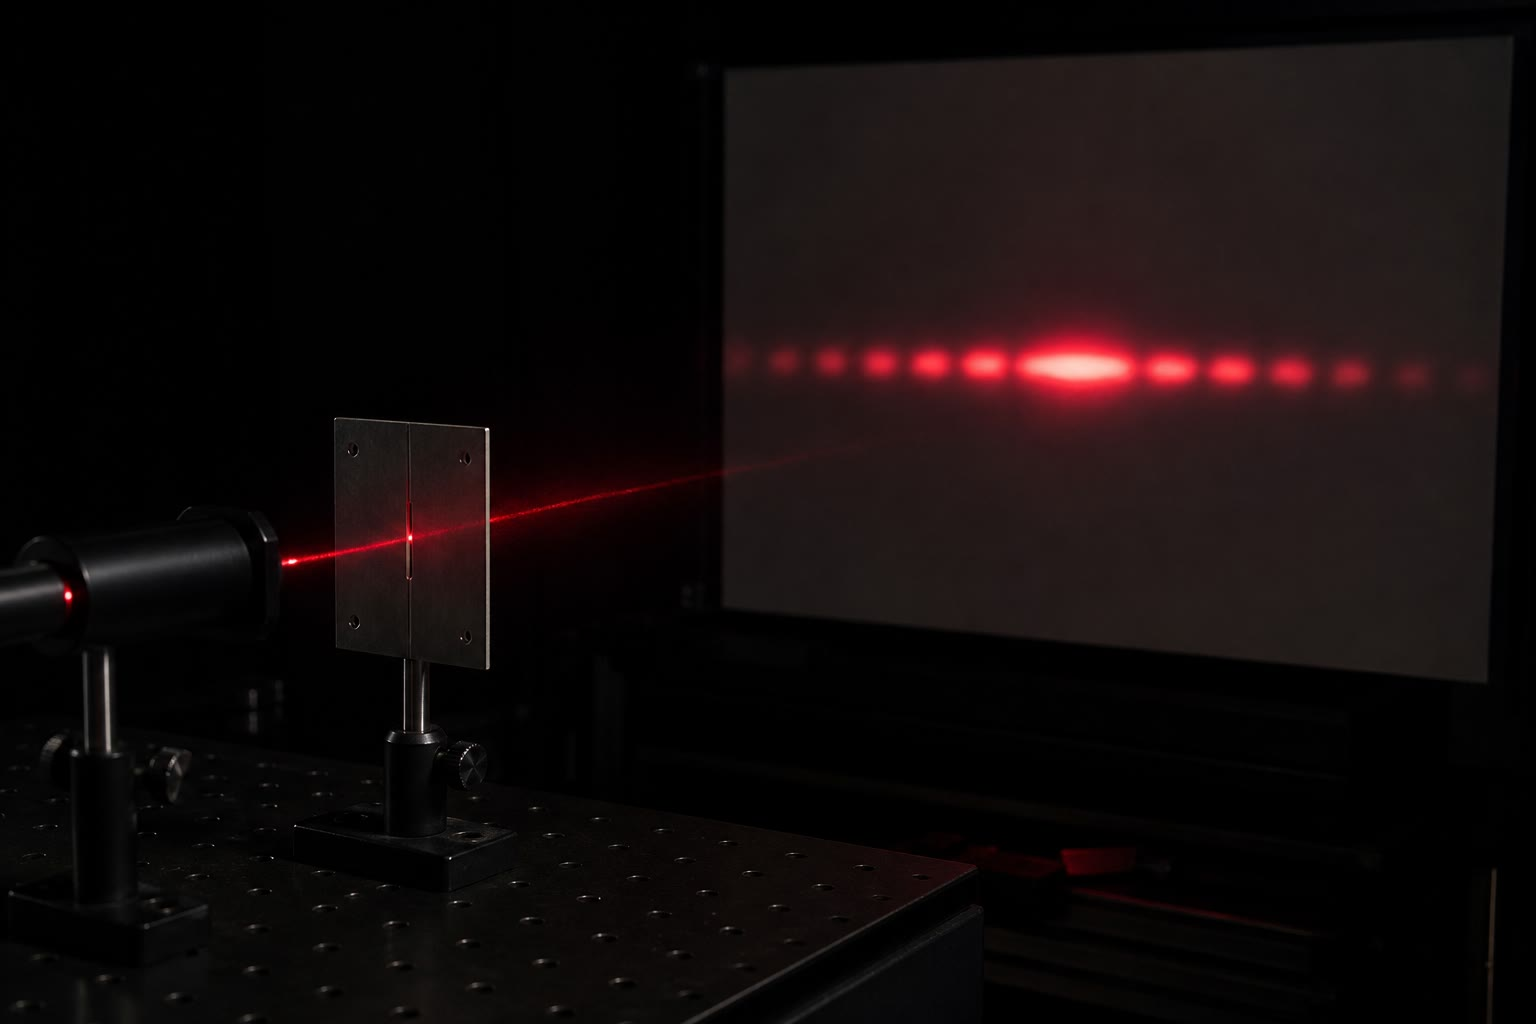
\includegraphics[width=0.58\linewidth]{images/book4/ai/b4-22-slit-diffraction-pattern.jpg}

{\small Een laserbundel door een smalle spleet: op het verre scherm de brede
heldere middenband en de flauwere, smallere nevenmaxima van het
fraunhoferpatroon.}
\end{omfigure}

\section{Vraagstuk: wat kan worden opgelost}

\begin{problem}[{Weekendvraagstuk --- de buigingsgrens op vier
schalen: het oog, een telescoop, een microscoop, en de laserbundel die
moet worden schoongemaakt voordat hij wordt gebruikt}]
\label{pb:b2:diffraction:1}

\medskip
\noindent\textbf{Deel I --- Het oog.}
Pupil $D = \qty{3}{mm}$ overdag, \qty{7}{mm} 's nachts;
$\lambda = \qty{550}{nm}$; de
kegeltjes van het netvlies liggen in de fovea \qty{2}{\micro m} uit elkaar,
de brandpuntsafstand
van het oog is \qty{17}{mm}.
\begin{enumerate}
  \item Hoekstraal van de \omterm{prop:b2:diffraction:airy}{airyschijf} overdag; haar lineaire straal op
        het netvlies; vergelijk met de afstand tussen de kegeltjes --- is
        het netvlies
        op de optiek afgestemd?
  \item Kleinste scheiding van twee punten die op \qty{25}{cm} wordt opgelost; op
        \qty{10}{m}; kunt u een tekst van \qty{1}{mm} op armlengte lezen?
  \item 's Nachts opent de pupil zich tot \qty{7}{mm}: buigingsgrens dan;
        waarom wordt het zien toch slechter (afwijkingen van de
        lens bij volle opening, staafjes grover dan kegeltjes)?
  \item Twee autokoplampen op \qty{1.5}{m} afstand: afstand waarop zij tot
        één licht versmelten.
  \item Een gaatje van \qty{1}{mm} voor het oog gehouden: wat doet de \omterm{def:b2:diffraction:huygens}{buiging},
        en waarom helpt een speldenprik een bijziend oog toch
        (scherptediepte)?
\end{enumerate}

\medskip
\noindent\textbf{Deel II --- De telescoop.}
Een telescoop van \qty{1}{m}, $f = \qty{10}{m}$, met een camera met pixels
van \qty{10}{\micro m};
$\lambda = \qty{550}{nm}$.
\begin{enumerate}[resume]
  \item Buigingsgrens in boogseconden; airystraal op de
        detector; pixels per \omterm{prop:b2:diffraction:airy}{airyschijf}.
  \item De dampkring vervaagt beelden tot \qty{1}{''}: hoeveel van het
        oplossend vermogen van de telescoop gaat verloren? Diameter van de
        telescoop waarvoor
        de buigingsgrens gelijk is aan de seeing.
  \item Adaptieve optiek verbetert de dampkring bij \qty{2.2}{\micro m}:
        buigingsgrens daar; waarom is het in het infrarood gemakkelijker?
  \item Een dubbelster met componenten op \qty{0.15}{''} afstand: opgelost met
        adaptieve optiek bij \qty{2.2}{\micro m}? Bij \qty{550}{nm} vanuit
        de ruimte?
  \item De maan is \qty{3.8e5}{km} ver: kleinste krater die deze telescoop
        zou kunnen oplossen (alleen \omterm{def:b2:diffraction:huygens}{buiging}); en de voetafdruk van een maanlander
        (\qty{4}{m})?
  \item Lichtopbrengst van de telescoop ten opzichte van het
        nachtoog (\qty{7}{mm}); wat levert dat op, en wat niet?
  \item Het licht van een ster door de vier spaken die de
        secundaire spiegel houden: beschrijf het beeld.
\end{enumerate}

\medskip
\noindent\textbf{Deel III --- De microscoop.}
Objectief met \omterm{prop:b2:guided-waves:fibre}{numerieke apertuur} $\mathrm{NA} = n\sin\alpha = 0.9$ (droog) of $1.4$
(olie), $\lambda = \qty{550}{nm}$; de opgeloste afstand is
$0.61\lambda/\mathrm{NA}$.
\begin{enumerate}[resume]
  \item Opgeloste afstand met elk objectief; aantal lijnparen
        per millimeter.
  \item Een bacterie van \qty{1}{\micro m} met inwendige structuur op
        \qty{0.2}{\micro m}: wat wordt met elk gezien? Een virus van
        \qty{0.1}{\micro m}?
  \item Abbe: een periodieke structuur met periode $d$ wordt alleen
        afgebeeld als haar
        eerste orden bij $\sin\theta = \lambda/d$ het objectief binnenkomen:
        kleinste $d$
        voor $\mathrm{NA} = 1.4$; vergelijk met $0.61\lambda/\mathrm{NA}$.
  \item Waarom verbetert olie tussen het preparaat en het objectief het
        oplossend vermogen?
  \item Ultraviolet bij \qty{250}{nm} en een elektronenmicroscoop bij \qty{4}{pm}:
        opgeloste afstanden in dezelfde formule (voor elektronen is de
        praktische NA \qty{0.01}{}): vergelijk.
  \item Een cel is doorzichtig: in helderveld is haar beeld leeg.
        Verklaar in twee zinnen wat het fasecontrastplaatje in het
        fouriervlak van het objectief doet.
\end{enumerate}

\medskip
\noindent\textbf{Deel IV --- De bundel.}
Een laser bij \qty{532}{nm}, bundeldiameter \qty{1.5}{mm}, moet tot
\qty{30}{mm} worden verbreed en schoongemaakt.
\begin{enumerate}[resume]
  \item Buigingshalfhoek van de ruwe bundel ($\sim1.22\lambda/D$); zijn
        diameter na \qty{100}{m} zonder optiek.
  \item Een lens met $f_1 = \qty{10}{mm}$ bundelt hem: diameter van de brandvlek;
        gekozen diameter van de speldenprik ($1.5\times$ de vlek).
  \item Een tweede lens met $f_2$ maakt bij \qty{30}{mm} weer evenwijdig:
        $f_2$; nieuwe
        buigingshoek; diameter na \qty{1}{km}.
  \item Stof van \qty{100}{\micro m} op de eerste lens buigt onder welke hoek;
        waar valt dat licht in het vlak van de speldenprik, en wat
        gebeurt ermee?
  \item De speldenprik laat $99\%$ van een gaussische bundel door: verloren
        vermogen, en
        waar het heen gaat.
  \item Waarom moet de verbrede bundel \emph{groter} zijn om evenwijdig te blijven
        (breng $\lambda/D$ in verband met de afstand waarover de bundel verdubbelt,
        $\sim D^2/\lambda$)?
  \item Vat de vier grenzen van dit vraagstuk samen in één tabel: opening,
        golflengte, $\lambda/D$, wat zij begrenst.
\end{enumerate}
\end{problem}
